%%%%%%%%%%%%%%%%%%%%%%%%%%%%%%%%%%%%%%%%%%%%%%%%%%%%%%%%%%%%%%%%%%%%%
% LaTeX Template: Project Titlepage Modified (v 0.1) by rcx
%
% Original Source: http://www.howtotex.com
% Date: February 2014
% 
% This is a title page template which be used for articles & reports.
% 
% This is the modified version of the original Latex template from
% aforementioned website.
% 
%%%%%%%%%%%%%%%%%%%%%%%%%%%%%%%%%%%%%%%%%%%%%%%%%%%%%%%%%%%%%%%%%%%%%%

\documentclass[12pt]{article}
\usepackage[a4paper]{geometry}
\usepackage[myheadings]{fullpage}
\usepackage{fancyhdr}
\usepackage{lastpage}
\usepackage{graphicx, wrapfig, subcaption, setspace, booktabs}
\usepackage[T1]{fontenc}
\usepackage[font=small, labelfont=bf]{caption}
\usepackage{fourier}
\usepackage[protrusion=true, expansion=true]{microtype}
\usepackage[english]{babel}
\usepackage{sectsty}
\usepackage{url, lipsum}

\newcommand{\HRule}[1]{\rule{\linewidth}{#1}}
\onehalfspacing
\setcounter{tocdepth}{5}
\setcounter{secnumdepth}{5}

%-------------------------------------------------------------------------------
% HEADER & FOOTER
%-------------------------------------------------------------------------------
\pagestyle{fancy}
\fancyhf{}
\setlength\headheight{15pt}
\fancyhead[L]{CHARM}
\fancyhead[R]{Carleton University}
\fancyfoot[R]{Page \thepage\ of \pageref{LastPage}}
%-------------------------------------------------------------------------------
% TITLE PAGE
%-------------------------------------------------------------------------------

\begin{document}
\bibliographystyle{ieeetr}

\title{ \normalsize \textsc{}
		\\ [2.0cm]
		\HRule{0.5pt} \\
		\LARGE \textbf{{Carleton High Altitude Radiometer}}\\
		\large \textbf{{Project Proposal}}\\
		\large \textbf{{Canadian Stratospheric Balloon Experiment Design Challenge}}
		\HRule{2pt} \\ [0.5cm]
		\normalsize \today \vspace*{2\baselineskip}\\
		
\includegraphics[scale=0.6]{Figures/CHARM.png}	\vspace*{2\baselineskip} \\
		\textsc{
		David Bascelli \quad Team Lead \\
		Jacob Booth \quad Sensor Lead \\
		}}
		
\date{}
	
\author{
		Carleton University \\
		}
	


\maketitle

\newpage

\tableofcontents
\newpage

\listoffigures
\newpage

\listoftables
\newpage

%-------------------------------------------------------------------------------
% Section title formatting
\sectionfont{\scshape}
%-------------------------------------------------------------------------------

%-------------------------------------------------------------------------------
% BODY
%-------------------------------------------------------------------------------

\section{Executive Summary}
Microwave remote sensing has been a common payload on earth observation satellites since the early days of space-flight. In as early as 1962, a radiometer on-board the Mariner 2 mission measured the surface temperature of Venus. 1968 Saw the first space-born earth observation radiometer on-board the  Cosmos 243 satellite, which measured atmospheric water vapour and global ice cover. Many different radiometer configurations can make a wide array of different geological, biological, and climate measurements. The CHARM project will design and manufacture a C-band balloon mounted microwave radiometer for the purpose of measuring soil moisture content over a large area. Soil moisture measurements are crucial in predicting local weather conditions and monitoring climate change. Incorporating soil moisture measurements into weather and climate models allows for more accurate medium term weather forecasts and can also give clues about future droughts, crop yields, and water resource management. Currently, most radiometric data comes from space-born radiometers, such as those on the SMAP or SMOS satellites. To achieve high resolution and accuracy, these space-born radiometers utilize cryogenic components, complex phased array or synthetic aperture technologies, and require large and very directional antennas. Our belief is that measurements of similar similar quality could be performed from a high altitude balloon at significantly reduced cost. 

\newpage

\section{Proposal}
\subsection{Scientific Objectives}

 Our scientific objective is to make low cost measurements of soil moisture content using a balloon born microwave radiometer. 

Balloon born radiometers even have some advantages to space-born radiometers, including reduced antenna directionality requirements and reduced atmospheric effects.

 
\subsection{Experiment Design}
\subsubsection{Outline}

\subsubsection{Antenna Selection and Fabrication}
The design and construction of the antenna system presents many challenges, both in our radiometer and in space 
based systems. Antennas must be highly directional (have a high gain), which typically requires them to be quite large and heavy. In addition, lower frequencies require bigger antennas. In fact, earlier iterations of the design 
operated at a much lower frequency to make the electronics simpler, however it would not have been possible to fit
the antenna. Therefore, antenna sizing is the defining constraint on this system.\\

There are two solutions under consideration for the design of the antenna. A single large antenna, or an antenna 
array. Using an array of radiometers, we can create a synthetic aperture radiometer (SAR). With this solution we
would likely measure at 1.4 GHz, reducing hardware expense and complexity. This would involve precisely placing
four to eight antennas around the base of the gondola. The individual antennas would only be 10 cm long, and
weight very little. Coax cable would then need to be routed back to the experiment case. The use of SAR is common
in space based installations, as it is far lighter then having a large dish \cite{skou1989microwave}. 
However, the placement of many antennas, and the routing of many cables through the gonadal would be 
problematic. In addition the signal processing required to get meaningful data from a SAR is incredibly complex
and difficult, making this solution undesirably. It is mentioned in the event that the second solution does 
not work.\\

The second solution is to use a large horn antenna which sticks out from the side of the gonadal as shown in 
figure \ref{fig:antenna}. While this has the advantage of being easier to implement and build, it is heavier 
and less accurate then SAR. The exact sizing of the antenna would have to be carefully chosen to be as big
as allowable (the larger the antenna, the better the accuracy will be), but at a minimum the large opening will
need to be 30 cm by 30 cm. The horn can also be a rectangular shape, do that it is as wide as the gonadal, but 
only sticks out by 30 cm. The horn antenna will contain two output pins, this will allow us to measure the
polarization of the incident radiation as well as its magnitude and spectrum \cite{constantine2005antenna}.
Being able to take these simultaneous measurements will improve results.\\
\begin{figure}
	\centering
	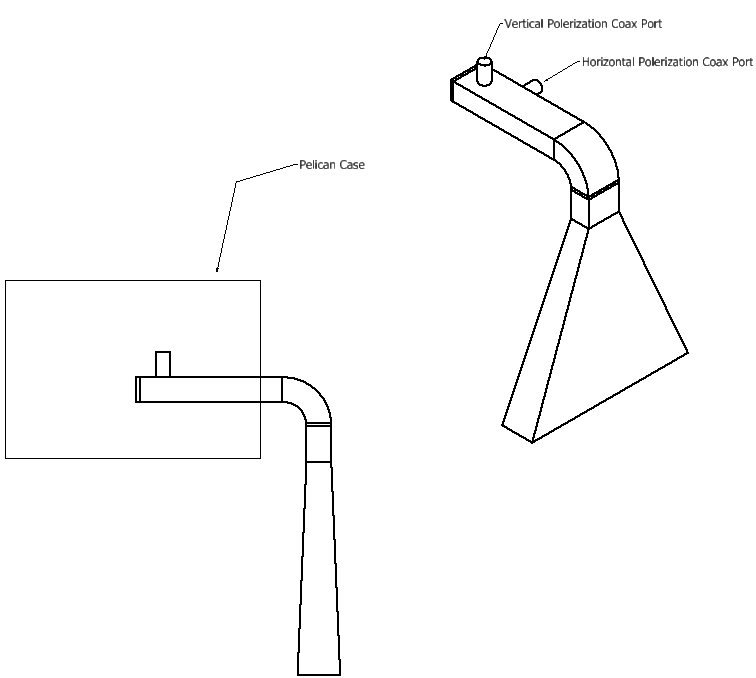
\includegraphics[width=0.5\linewidth]{Figures/rough_antenna.png}
	\label{fig:antenna}
	\caption{Horn antenna}
\end{figure}
The graph shown in figure \ref{fig:antenna_direction} shows the directivity of the antenna shown in figure
\ref{fig:antenna} (note that this is just an concept an not the final design). The directivity is high in 
the dimension where the antenna is large. This means that if we have a wide and thin antenna we are going to 
be scanning narrow bands along the ground. 
\begin{figure}
	\centering
	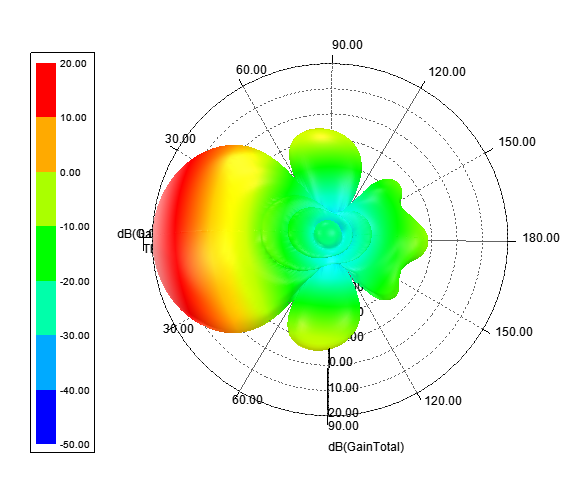
\includegraphics[width=0.5\linewidth]{Figures/antenna_gain.png}
	\label{fig:antenna_direction}
	\caption{Horn antenna directivity}
\end{figure}
One way of constructing the antenna is to have large copper sheets cut into shape then soldered together. While
this is fairly easy, it is imprecise and the resulting antenna is heavy. Another solution being investigated is
to 3D print the antenna, then chemically copper plate it. This will allow us to create more complicated geometry
and be much lighter then something made of solid copper. In house electroplating is being investigated for 
reduced cost, but the process in difficult and requires the development of procedures and techniques
\cite{bryancera2014}. Alternatively, a third party can be payed to electroplate our 3D print, though it would 
cost more.

\subsubsection{Radiometer Block Diagram}
David
\subsubsection{Attitude Determination}
Jacob
\subsubsection{Experimental Procedures}
David
\subsubsection{Resources}
David
\subsubsection{Technical Risk Assessment}
Jacob
\begin{enumerate}
\item Human
\cite{omar_el-kassaby_abdelghaffar_2017}
\item Technical and Environmental
\end{enumerate}
\subsection{Management}
David
\subsubsection{Team Structure}
\subsubsection{Project Time-line}
\subsubsection{Budget}
\subsubsection{Managerial Risk Assessment}

\subsection{Outreach}
Jacob
\subsubsection{Public Outreach}
\subsubsection{Academic Outreach}

\section{Conclusion}

%-------------------------------------------------------------------------------
% REFERENCES
%-------------------------------------------------------------------------------
\newpage
\section{References}

\bibliography{library}

\section{Appendix}


\end{document}
